\documentclass{article}

\usepackage{graphicx}
\usepackage{tikz}
\usepackage{tikzsymbols}
\usetikzlibrary{calc,patterns,shapes.geometric}
\pagestyle{empty}
\usepackage[margin=0pt]{geometry}
\geometry{papersize={14in,12in}}

\def\centerarc[#1](#2)(#3:#4:#5){\draw[#1] ($(#2)+({#5*cos(#3)},{#5*sin(#3)})$) arc (#3:#4:#5);}

\begin{document}
	\begin{figure}
		\centering
		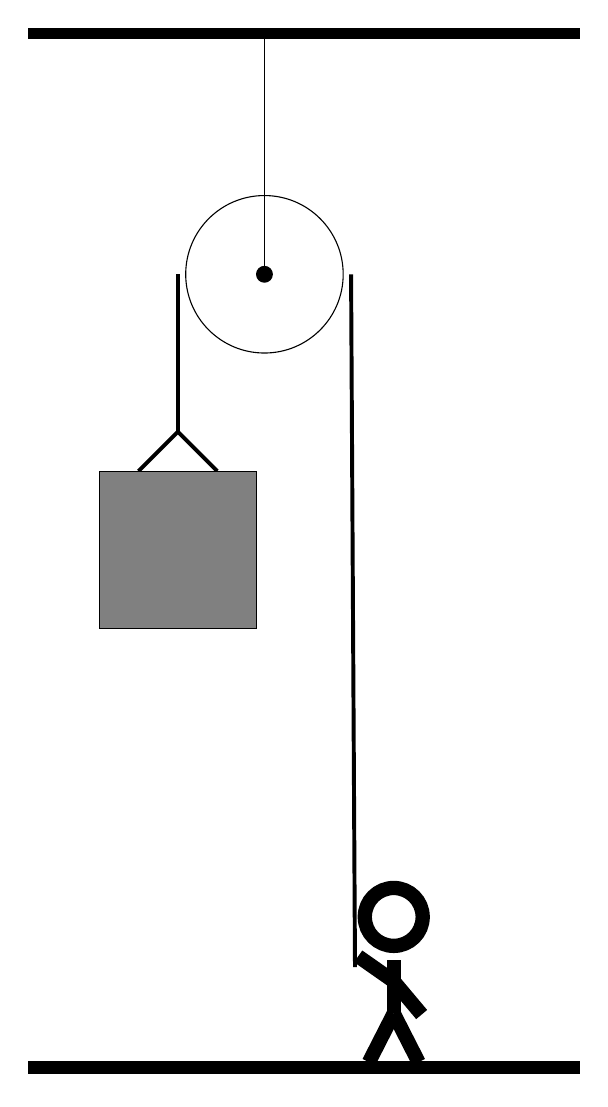
\begin{tikzpicture}
			%%%%% START %%%%%
			\draw[fill=black] (-2, 10) rectangle (5, 10.125);
			
			\draw (1, 7) circle (1);
			\draw[fill=black] (1, 7) circle (0.1);
			\draw (1, 10) -- (1, 7);
			
			\draw[line width=0.5mm] (-0.6, 4.5) -- (-0.1, 5.0) -- (0.4, 4.5);
			\draw[fill=black!50] (-1.1, 4.5) rectangle (0.9, 2.5);
			
			\draw[line width=0.5mm] (-0.1, 7) -- (-0.1, 5.0);
			\centerarc[line width=0.5mm](1, 7)(0:180:1.1);
			\draw[line width=0.5mm](2.1, 7) -- (2.15, -1.8);
			
			\node at (2.6, -1.9) {\Strichmaxerl[10][-35][-50]};
			
			\draw[fill=black] (-2, -3) rectangle (5, -3.15);
			%%%%% END %%%%%
		\end{tikzpicture}
	\end{figure}	
\end{document}